\documentclass{article}
\usepackage{../../Self_Style}

\title{Phys 20AL Week 6 Lab Report: Driven Harmonic Oscillator}
\author{Zih-Yu Hsieh}
\date{\today}

\begin{document}
\maketitle

\tableofcontents

\newpage

\section{Introduction}
When given a damped harmonic oscillator with natural frequency $w_0$ and damping constant $\gamma$, if it's driven by a force of the form $F_0 \cos(w t)$ (where $w$ is the driven frequency), then after a long time (with the system reaches steady state), the position is given with the following function:
\begin{align}
    x\approx \frac{F_0/m}{\sqrt{(w_0^2-w^2)^2+4\gamma^2w^2}}\cos(wt-\delta),\quad A=\frac{F_0/m}{\sqrt{(w_0^2-w^2)^2+4\gamma^2w^2}}, \quad \delta =\arctan\left(\frac{2\gamma w}{w_0^2-w^2}\right)
\end{align}
Where $A$ denotes the maximum amplitude, and $\delta$ denotes the phase difference. The goal of this experiment is to observe if the experimental data fit with such theoretical prediction, and furthermore extract the damping constant $\gamma$ based on the collected data of amplitude, frequency, and phase difference.

\section{Experimental Setup}
The equipments included: A large stand (with multiple clamps provided), a heavy mass of $0.5$ kg (used as driven source of the harmonic oscillator), metal wire, multiple strings (total of 12), multiple light masses (total of 11, used as pendulums), scissors, tapes, two meter sticks, and phones.

The setup followed the steps below:
\begin{itemize}
    \item[1.] Tie the metal wire horizontally on the stand, and ensure it's tight enough.
    \item[2.] Use one of the strings to tie the heavy mass (0.5 kg) onto the metal wire (near one end of the wire), and tape it to ensure the metal wire would obtain some rotational motion when the heavy mass is swinging.
    \item[3.] Tie the light masses onto the wire. Ensure that they're spaced (so the pendulum motion would affect each other), while also close enough to the heavy mass (so the driven force caused by the heavy mass wouldn't be dissipated). Also, keep in mind of making each light mass pendulum with a different length, and with at least one having the same length as the heavy mass.
    \item[4.] Setup the two meter sticks below the pendulums: Fix one directly under the heavy mass, and fix the other meter stick directly under the light mass that's the farthest away from the heavy mass.
    \item[6.] Fix the phone at the other end of the stand, making sure the camera captures all pendulums, having all the masses are aligned in the center, and also including the meter sticks in the view of the camera. 
\end{itemize}

\begin{figure}[h!]
    \centering
    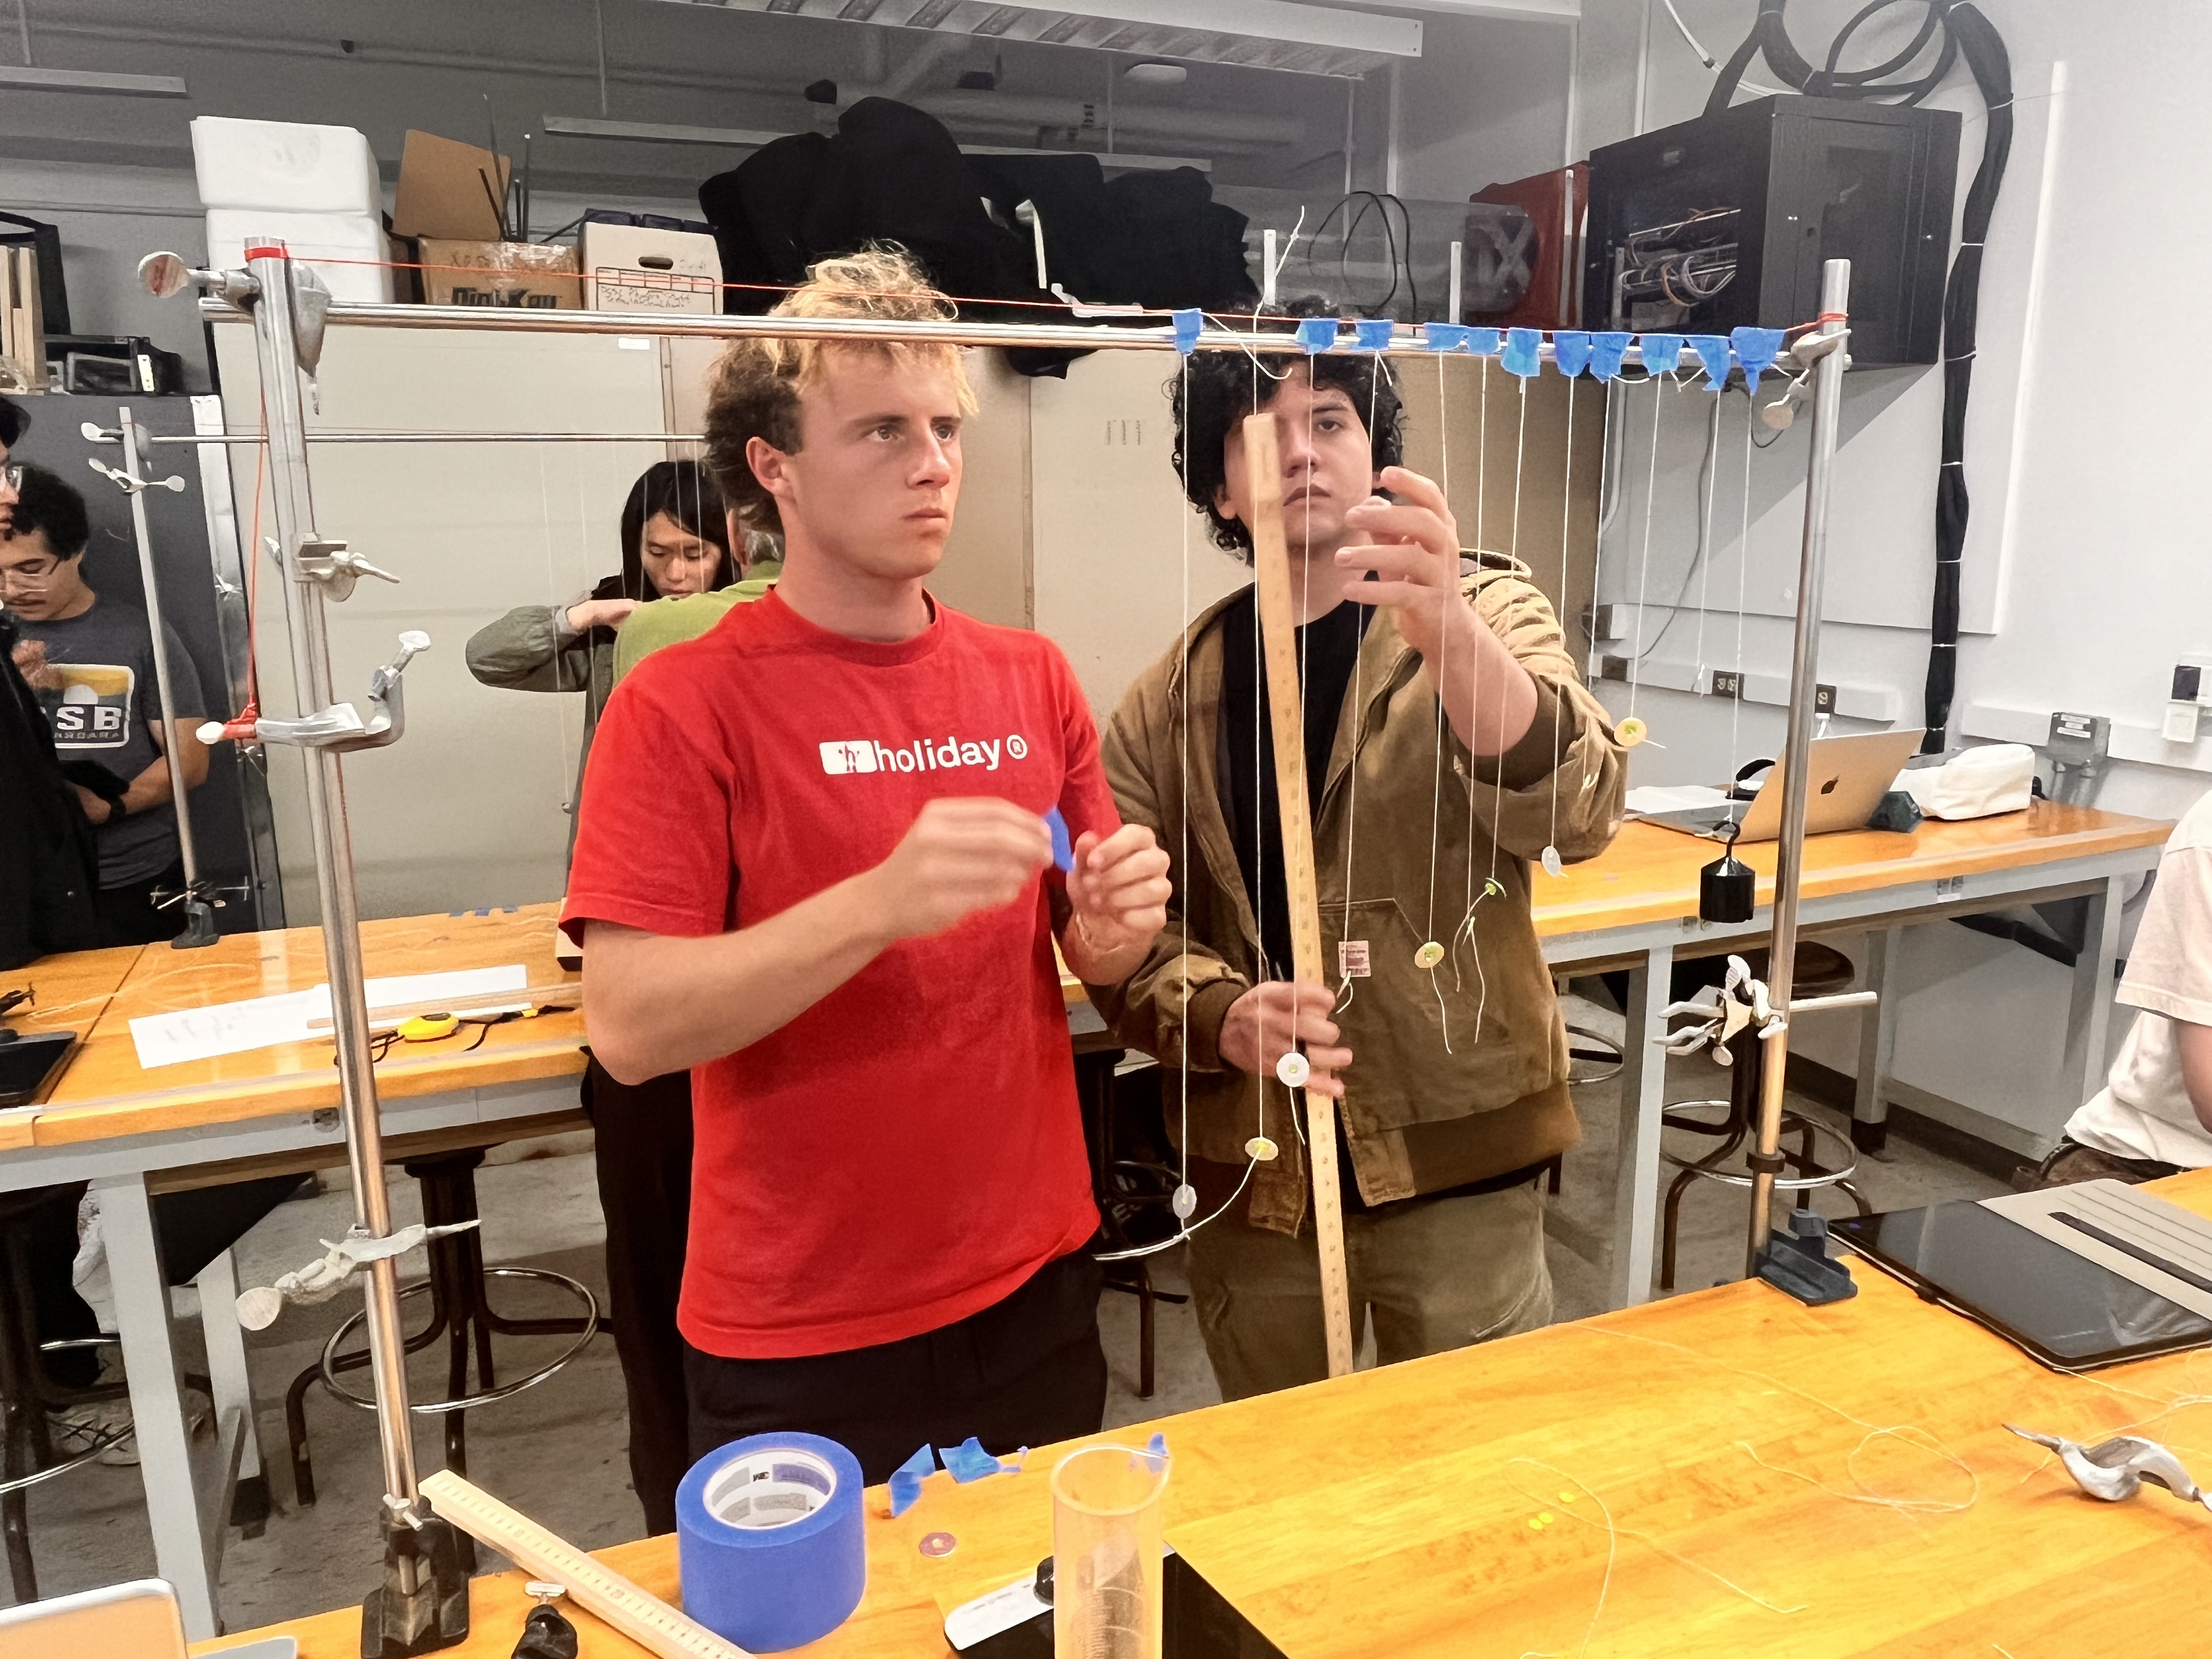
\includegraphics[width=60mm]{lab_setup_6.png}
    \caption{The Lab Setup Picture}
\end{figure}

\newpage

\section{Quantity to Measure and Method of Measurement}
In this experiment, one recorded a total of three trials. It is aimed to measure two quantities: The amplitudes of all the pendulum, and the phase difference.

For both amplitudes and phase difference, whole experimental process were recorded at stable state using camera. Then, the meter stick will serve as a metric to measure the amplitude of each pendulum; also, the time stamp of the video recording served as a source for measuring the time difference between the moment when each pendulum reaches maximum amplitude (vs. the moment when the driven pendulum reaches its maximum).

\hfil

\section{Experimental Procedure}
The procedure is as below:
\begin{itemize}
    \item[1.] Put the whole system at static equilibrium (having none of the pendulums actually moving), and raise the heavy mass to about $10$ cm away from equilibrium.
    \item[2.] Release the heavy mass pendulum, and wait until the system to reach a stable state.
    \item[3.] When the system reaches stable state, start recording, and let all the pendulums finish at least 5 to 6 cyclees.  
    \item[4.] Repeat Step 1 to 3 for a total of three trials. 
\end{itemize}

\newpage

\section{Experimental Data}
Here are the experimental data separated by trials.

\subsection{Trial 1}
\begin{table}[h!]
\centering
\caption{Trial 1 Data}
\begin{tabular}{rrrrrr}
\toprule
 omega &  omega\_0 &  x\_max &  delta &  x\_max\_error &  delta\_err \\
\midrule
 4.669 & 6.107 & 1.537 & 0.504 & 0.237 & 0.264 \\
 4.669 & 5.681 & 1.174 & 0.298 & 0.308 & 0.084 \\
 4.669 & 5.317 & 2.082 & 0.306 & 0.039 & 0.060 \\
 4.669 & 4.946 & 2.102 & 0.260 & 1.101 & 0.098 \\
 4.669 & 4.788 & 3.786 & 0.754 & 0.188 & 0.254 \\
 4.669 & 4.685 & 6.486 & 0.398 & 0.572 & 0.144 \\
 4.669 & 4.549 & 11.520 & 1.877 & 1.949 & 0.132 \\
 4.669 & 4.465 & 7.851 & 3.103 & 0.614 & 0.080 \\
 4.669 & 4.197 & 3.196 & 2.424 & 0.789 & 0.359 \\
 4.669 & 4.050 & 1.000 & 3.422 & 0.423 & 0.203 \\
\bottomrule
\end{tabular}
\end{table}
\begin{figure}[h!]
    \centering
    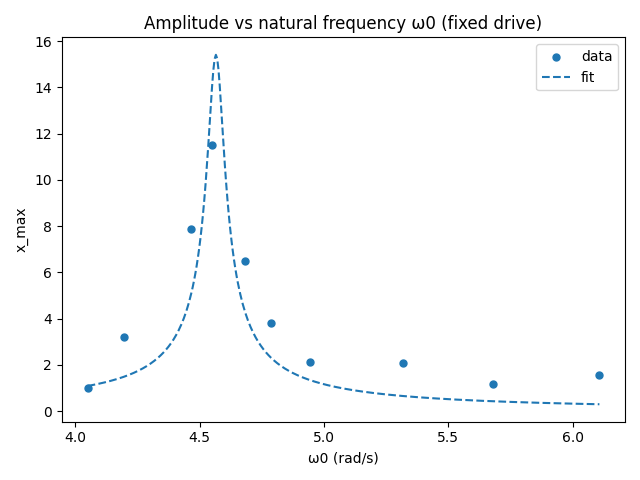
\includegraphics[width=100mm]{Amplitude 1.png}
\end{figure}
\begin{figure}[h!]
    \centering
    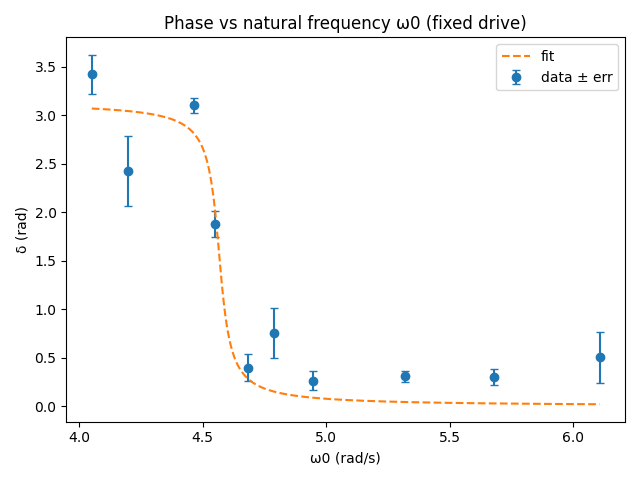
\includegraphics[width=100mm]{Phase 1.png}
\end{figure}

\newpage

\subsection{Trial 2}
\begin{table}[h!]
\centering
\caption{Trial 2 Data}
\begin{tabular}{rrrrrr}
\toprule
 omega &  omega\_0 &  x\_max &  delta &  x\_max\_error &  delta\_err \\
\midrule
 4.669 & 6.107 & 1.061 & 0.748 & 0.237 & 0.264 \\
       & 5.681 & 1.122 & 0.284 & 0.308 & 0.084 \\
       & 5.317 & 2.082 & 0.173 & 0.039 & 0.060 \\
       & 4.946 & 1.012 & 0.334 & 1.101 & 0.098 \\
       & 4.788 & 3.458 & 0.551 & 0.188 & 0.254 \\
       & 4.685 & 7.326 & 0.141 & 0.572 & 0.144 \\
       & 4.549 & 12.920 & 1.808 & 1.949 & 0.132 \\
       & 4.465 & 9.088 & 2.947 & 0.614 & 0.080 \\
       & 4.197 & 1.798 & 3.011 & 0.789 & 0.359 \\
       & 4.050 & 0.500 & 3.412 & 0.423 & 0.203 \\
       & 3.906 & 1.700 & 3.926 & 0.294 & 0.681 \\
\bottomrule
\end{tabular}
\end{table}
\begin{figure}[h!]
    \centering
    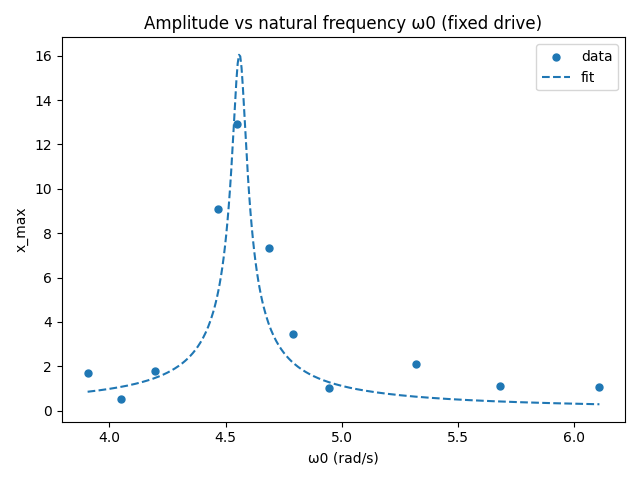
\includegraphics[width=100mm]{Amplitude 2.png}
\end{figure}
\begin{figure}[h!]
    \centering
    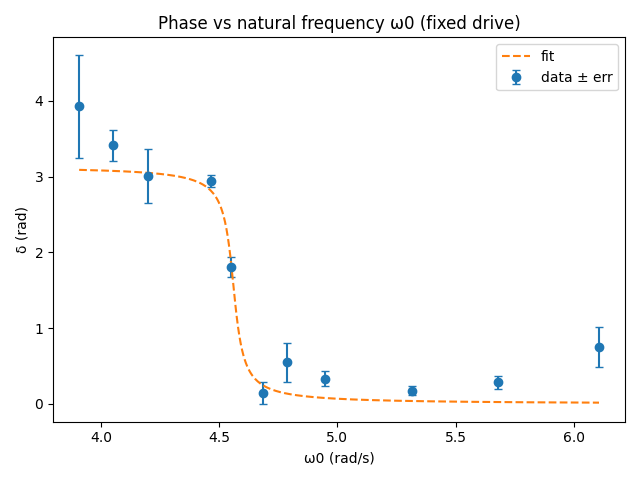
\includegraphics[width=100mm]{Phase 2.png}
\end{figure}

\newpage

\subsection{Trial 3}
\begin{table}[h!]
\centering
\caption{Trial 3 Data}
\begin{tabular}{rrrrrr}
\toprule
 omega &  omega\_0 &  x\_max &  delta &  x\_max\_error &  delta\_err \\
\midrule
 4.669 & 6.107 & 1.012 & 0.107 & 0.237 & 0.264 \\
       & 5.681 & 1.800 & 0.114 & 0.308 & 0.084 \\
       & 5.317 & 2.000 & 0.186 & 0.039 & 0.060 \\
       & 4.946 & 3.693 & 0.099 & 1.101 & 0.098 \\
       & 4.788 & 3.902 & 0.144 & 0.188 & 0.254 \\
       & 4.685 & 5.935 & 0.059 & 0.572 & 0.144 \\
       & 4.549 & 16.172 & 2.115 & 1.949 & 0.132 \\
       & 4.465 & 7.727 & 3.126 & 0.614 & 0.080 \\
       & 4.197 & 1.340 & 3.284 & 0.789 & 0.359 \\
       & 4.050 & 1.536 & 2.987 & 0.423 & 0.203 \\
       & 3.906 & 1.000 & 2.275 & 0.294 & 0.681 \\
\bottomrule
\end{tabular}
\end{table}
\begin{figure}[h!]
    \centering
    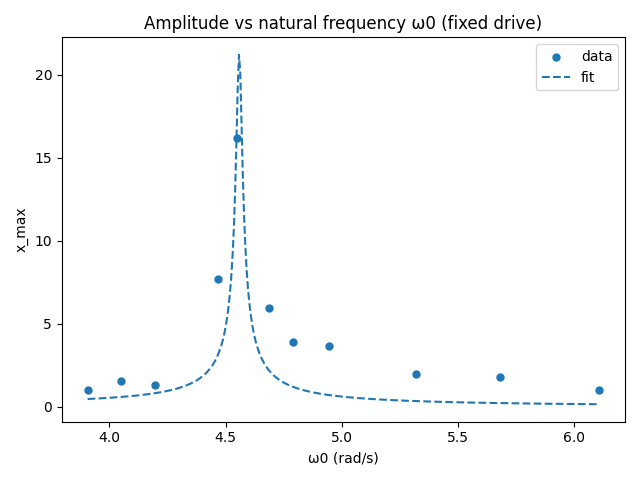
\includegraphics[width=100mm]{Amplitude 3.png}
\end{figure}
\begin{figure}[h!]
    \centering
    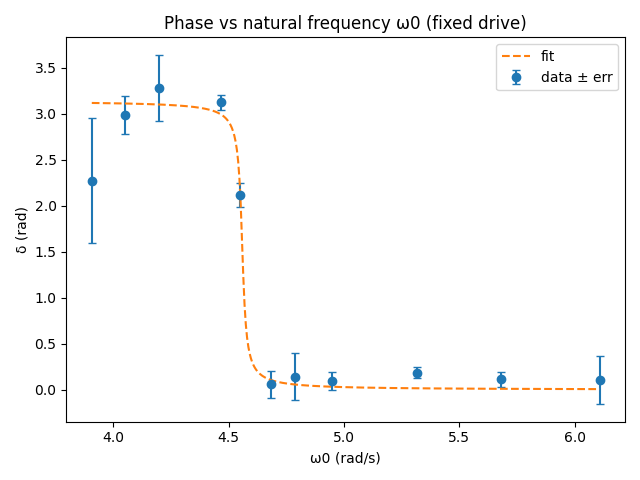
\includegraphics[width=100mm]{Phase 3.png}
\end{figure}


\end{document}